\documentclass[aps,prd]{revtex4-1}

\usepackage{hyperref} \usepackage{amsmath} \usepackage{amssymb}
\usepackage{graphicx} \usepackage{color}

\newcommand{\order}[1]{\mathcal{O}\left( #1 \right)}
\newcommand{\fixme}[1]{\textbf{FIXME: #1}}
\newcommand{\mathset}[1]{\left\{ #1 \right\}}

\newcommand{\xmin}{x_\mathrm{min}}

\newcommand{\ilya}[1]{{\color{red} \bf #1}}
\newcommand{\will}[1]{{\color{blue} \bf #1}}
\newcommand{\jon}[1]{{\color{orange} \bf #1}}

\DeclareMathOperator{\erf}{erf}

\begin{document}

\title{Bayesian Rate Estimation}

\author{Will M. Farr} \email{w-farr@northwestern.edu}
\homepage{http://faculty.wcas.northwestern.edu/will-farr/}
\affiliation{Center for Interdisciplinary Exploration and Research in
  Astrophysics\\ Department of Physics and Astronomy\\ Northwestern
  University, 2145 Sheridan Road, Evanston, IL 60208}
%\affiliation{Northwestern University and CIERA}

\author{Jonathan R. Gair} \email{jrg23@cam.ac.uk}
\affiliation{Institute of Astronomy\\University of
  Cambridge\\Madingley Road, Cambridge CB3 0HA\\United Kingdom}

\author{Ilya Mandel} \email{imandel@star.sr.bham.ac.uk}
\homepage{http://www.sr.bham.ac.uk/~imandel} \affiliation{School of
  Physics and Astronomy\\University of Birmingham\\Edgbaston B15 2TT
  Birmingham\\United Kingdom}
%\affiliation{University of Birmingham}


\begin{abstract}
  We show how to obtain a Bayesian estimate of the rate of signal
  events from a set of signal and background events when the shapes of
  the signal and background distributions are known, can be estimated,
  or approximated; our method works well even if the foreground and
  background event distributions overlap significantly.  We give
  examples of determining the rates of gravitatonal-wave events in the
  presence of background triggers from a template bank when noise
  parameters are known and/or can be fit from the trigger data.  We
  also give an example of determining globular-cluster shape and
  location parameters from an observation of a stellar field that
  contains a non-uniform background density of stars superimposed on
  the cluster stars.
\end{abstract}

\maketitle

\section{Introduction}

\fixme{Introduce the necessity of estimating rates, prior work (like
  \cite{Biswas2009}), Bayesian inference.}
  
Difficulty of measuring rate in presence of background

Want to add more than just the loudest event (cf. loudest event
statistic)

Unknown background distribution, $\Lambda$

Cf. number of gold-plated detections in sensitive volume --
frequentist approach OK if tons of events, otherwise need this.


\section{Model}

We assume that we are presented with a data set of $N$ events that
exceed a pre-specified threshold in ranking statistic, $x_{min}$.
Each event may be due to either a signal of interest or an
uninteresting background.  Each event is associated with a ranking
statistic, $x$.  Our data set therefore consists of the ranking
statistics for the set of events:
\begin{equation}
  d = \mathset{ x_i | i = 1, \ldots, N } .
\end{equation}
The number of events $N$ is also part of the observed data, but we
separate out $N$ and the observed ranking statistics, $d$, for
convenience. We can choose how to label our events. Ultimately we will
label the events in order of ranking statistic, i.e., $x_1 < x_2 <
\cdots < x_N$, but some of the derivations that follow are simpler if
the events are ordered by time of arrival. We will use $d$ to denote
ranking statistic-ordered events, and $d_{\rm to}$ to denote
time-ordered events.

We assume that both the foreground and background events are samples
from an inhomogeneous Poisson process with respective differential
rates
\begin{equation}
  \frac{dN_f}{dx} = f(x, \theta)
\end{equation}
and
\begin{equation}
  \frac{dN_b}{dx} = b(x, \theta),
\end{equation}
where the $\theta$ argument represents additional ``shape'' parameters
that may affect the distribution, and for which we will eventually
fit.  The cumulative rates of the two processes are therefore
\begin{equation}
  F(x,\theta) \equiv \int_{-\infty}^x ds\, f(s, \theta)
\end{equation}
and
\begin{equation}
  B(x,\theta) \equiv \int_{-\infty}^x ds\, b(s,\theta).
\end{equation}
The assumption that the foreground and background events form an
inhomogeneous Poisson process implies
\begin{enumerate}
\item \label{prop:Poisson} The number of events in any range of
  ranking statistics, $x \in [x_1, x_2]$ is Poisson distributed with
  rate $F(x_2, \theta) - F(x_1,\theta)$ or $B(x_2,\theta) -
  B(x_1,\theta)$.
\item The numbers of events in non-overlapping ranges of ranking
  statistics are independent.
\item The probability of exactly one foreground event between $x$ and
  $x+h$ is given by
  \begin{equation}
    P(n = 1 \in [x, x+h]) = f(x,\theta) h + \order{h^2}.
  \end{equation}
  and similarly for background events.
\item The probability of two or more events in a small range of
  ranking statistic is negligible
  \begin{equation}
    P(n = 2 \in [x, x+h]) = \order{h^2}.
  \end{equation}
\end{enumerate}
The foreground and background rates can in general depend on several
parameters; the goal of our analysis is to determine the posterior
probability distributions for these parameters that are implied by the
data.  At the least, we will want to know the overall amplitude of the
foreground and background rates.  Let
\begin{equation}
  f(x,\theta) = R_f \hat{f}(x,\theta'),
\end{equation}
and
\begin{equation}
  b(x, \theta) = R_b \hat{b}(x, \theta'),
\end{equation}
where $\hat{F}(\infty, \theta') = \hat{B}(\infty, \theta') = 1$, and
$\theta' = \theta \setminus \{R_{f}, R_{b} \}$.  Then $R_f \equiv
F(\infty,\theta)$ and $R_b \equiv B(\infty,\theta)$ are the total
number of foreground and background events expected and $\hat{f}(x,
\theta')$ and $\hat{b}(x, \theta')$ are the likelihood of obtaining an
event with ranking statistic $x$ under the foreground and background
distributions.  In what follows, we will drop the prime, using
$\theta$ to denote all parameters of the rate distributions except
$R_f$ and $R_b$.

We do not know a priori which of the events are foreground and which
are background.  For each event, we introduce a flag, $f_i$, which is
either 0 (background) or 1 (foreground).  These ``state'' flags are
parameters in our model, along with $R_f$, $R_b$, and $\theta$.  We
can marginalize over our uncertainty in the state of any given event
by summing posteriors over $f_i = \mathset{0,1}$.

Assuming time-ordered data, $d_{\rm to}$, in the following, Bayes'
theorem relates the posterior probability of the state flags, rates,
and shape parameters, $p\left(\mathset{f_i}, R_f, R_b, \theta | d_{\rm
  to}, N \right)$, the likelihood of the data, $p\left( d_{\rm to} |
\mathset{f_i}, N, R_f, R_b, \theta\right)$, and the prior probability
of state flags, rates and shape parameters before any data are
obtained, $p\left( \mathset{f_i}, N, R_f, R_b, \theta\right)$:
\begin{equation}
  \label{eq:Bayes}
  p\left(\mathset{f_i}, R_f, R_b, \theta | d_{\rm to}, N \right) =
  \frac{p\left( d_{\rm to} | \mathset{f_i}, N, R_f, R_b, \theta\right)
    p\left(\mathset{f_i}, N, R_f, R_b, \theta\right)}{p(d_{\rm to},
    N)}.
\end{equation}
The normalization constant, called the evidence, $p(d_{\rm to}, N)$,
is independent of the state flags, rates, and shape parameters.

Each foreground event is drawn from the probability distribution
$\hat{f}$ and each background event is drawn from the probability
distribution $\hat{b}$.  The events are independent of each other.
Therefore, the likelihood of the data is
\begin{equation}
  p\left( d_{\rm to} | \mathset{f_i}, N, R_f, R_b, \theta\right) =
  \left[ \prod_{\mathset{i | f_i = 1}} \hat{f}\left(x_i, \theta\right)
    \right] \left[ \prod_{\mathset{i | f_i = 0}} \hat{b}\left( x_i,
    \theta\right) \right].
\end{equation}
This is the probability that the first observed event is a
fore/background event (if $f_i=1,0$) with ranking statistic $x_1$ and
the second observed event is a fore/background event (if $f_i=1,0$)
with ranking statistic $x_2$ etc. If the events are ordered by ranking
statistic the corresponding expression is more complicated, since
$x_1$ is now the event from foreground or background, with the
smallest ranking statistic etc. We will return to the
statistic-ordered case later.

%The prior distribution can be factorized as
%\begin{equation}
%  \label{eq:combined-flag-rate-prior}
%  p\left(\mathset{f_i}, R_f, R_b, \theta\right)  = p\left(
%   \mathset{f_i} | R_f, R_b, \theta\right)p(R_f, R_b, \theta).
%\end{equation}
%The first term is not actually a ``prior'' in the usual sense; the
%conditional probability of the flags $\mathset{f_i}$ on the rates is given
%by
%\begin{equation}
%  \label{eq:flag-conditional-prior}
%  p\left(\mathset{f_i} | R_f, R_b, \theta\right) = \frac{R_f^{N_f}
%    R_b^{N_b}}{N_f! N_b!} \exp\left[ - \left(R_f + R_b\right) \right]
%  N_f! N_b! = R_f^{N_f}R_b^{N_b} \exp\left[ - \left(R_f + R_b\right) \right],
%\end{equation}
%where $N_f$ and $N_b$ are the number of foreground and background
%events.  This expression follows from Property \ref{prop:Poisson} of
%inhomogeneous Poisson processes and the $N_f! N_b!$ different ways of
%assigning foreground and background flags to events for fixed $N_f$,
%$N_b$.  
%
%\ilya{[I agree with the final result, but I find this way of deriving
%    it to be confusing.  First of all, the number of ways to assign
%    flags to events for fixed $N_f$ and $N_b$ is $N!/(N_f! N_b!)$, not
%    $N_f! N_b!$ as written.  Secondly, you are computing the
%    probability of having a particular ordered list of flags, so
%    there's no reason to consider different permutations.  Thirdly,
%    you are not properly including the fact that the length of the
%    flags vector must be exactly $N$, the total number of data points.
%    (Well, you have the right result, so you are obviously doing these
%    things properly, but the explanation just doesn't seem clear to
%    me. :) ) I would make that $N$ explicit, by writing Eq.~(12) as

The prior distribution can be factorized as
\begin{equation}
  \label{eq:combined-flag-rate-prior}
  p\left(\mathset{f_i}, N, R_f, R_b, \theta\right) = p\left(
  \mathset{f_i} | N, R_f, R_b\right) p\left(N |R_f, R_b\right)
  p\left(R_f, R_b, \theta\right) = p\left( \mathset{f_i},N | R_f,
  R_b\right) p\left(R_f, R_b, \theta\right).
 \end{equation}
 
The probability that the $i$'th state flag is $f_i=1$ is given by
$R_f/(R_f+R_b)$, while the probability that it is zero is
$R_b/(R_f+R_b)$, provided the data are time-ordered as we have
assumed.  Then
\begin{equation}
p\left( \mathset{f_i} | N, R_f, R_b\right) = \prod_{\mathset{i|f_i=1}}
\left(\frac{R_f}{R_f+R_b}\right) \prod_{\mathset{i|f_i=0}}
\left(\frac{R_b}{R_f+R_b}\right) =
\left(\frac{R_f}{R_f+R_b}\right)^{N_f}
\left(\frac{R_b}{R_f+R_b}\right)^{N_b},
\end{equation}
where $N_f$ and $N_b$ are the numbers of foreground and background
flags, $N_f+N_b=N$.  Meanwhile,
\begin{equation}
p\left(N |R_f, R_b\right) = \frac{\left(R_f+R_b\right)^N}{N!}
e^{-(R_f+R_b)},
\end{equation}
since the distribution of total event number is a Poisson process with
rate $R_f+R_b$.  Combining these yields the conditional probability of
the flags on the rates:
\begin{equation}
  \label{eq:flag-conditional-prior}
  p\left(\mathset{f_i},N | R_f, R_b\right) = \frac{R_f^{N_f}
    R_b^{N_b}}{N!} \exp\left[ - \left(R_f + R_b\right) \right].
\end{equation} 


The second term in Eq.~\eqref{eq:combined-flag-rate-prior} is a
traditional prior.  Because the rate parameters enter the posterior in
the same form as Poisson rates, we choose here the Poisson Jeffreys
prior on rates \citep{Jeffreys1946}, independent of the shape
parameters
\begin{equation}
  p\left( R_f, R_b, \theta\right) = \alpha \frac{1}{\sqrt{R_f R_b}}
  p(\theta),
\end{equation}
where $\alpha$ is a normalisation constant, but of course other
choices are possible.  This choice has the advantage that the prior is
normalizable as $R_f, R_b \to 0$, and the exponentials in
Eq.~\eqref{eq:flag-conditional-prior} regularize the posterior as
$R_f, R_b \to \infty$.

Putting everything together, the posterior is
\begin{equation}
  \label{eq:posterior}
  p\left( \mathset{f_i}, R_f, R_b, \theta | d_{\rm to},N \right) =
  \frac{\alpha}{p(d_{\rm to},N)\,N!} \left[ \prod_{\mathset{i | f_i =
        1}} R_f \hat{f}\left(x_i, \theta\right) \right] \left[
    \prod_{\mathset{i | f_i = 0}} R_b \hat{b}\left( x_i, \theta\right)
    \right] \exp\left[ - \left(R_f + R_b\right) \right]
  \frac{p(\theta)}{\sqrt{R_f R_b}}
\end{equation}
When sampling the posterior, the first term can be omitted and the
equals sign replaced by proportionality, since it is independent of
the parameters of interest, but we have kept this term explicitly so
that we can see the equivalence to ranking-statistic ordered
data. Once data have been observed, there is a unique loudness
ordering and time ordering of those events, and so there is a one to
one correspondence between a time-ordered posterior $p\left(
\mathset{f_i}, R_f, R_b, \theta | d_{\rm to},N \right)$ and the
corresponding statistic-ordered posterior $ p\left( \mathset{f_i},
R_f, R_b, \theta | d,N \right)$, which means $p\left( \mathset{f_i},
R_f, R_b, \theta | d,N \right) = p\left( \mathset{f_i}, R_f, R_b,
\theta | d_{\rm to},N \right)$. However, the evidence $p(d,N) =
N!\,p(d_{\rm to},N)$, since there are $N!$ ways in which $N$ events
can be ordered in time and would have the same set of ranking
statistics.

Not surprisingly, this ranking-statistic ordered posterior can be
computed directly by assuming that the flags, $\mathset{f_i}$, are
un-observed data and treating the sets $\mathset{x_i | f_i = 1}$ and
$\mathset{x_i | f_i = 0}$ as samples from an inhomogeneous Poisson
process.  For an inhomogeneous Poisson process with rate function
$r(y)$ (cumulative rate $R(y)$), the likelihood of a set of samples
$\mathset{y_i}$ is given by
\begin{multline}
  p\left( \mathset{y_i} | r \right) \,{\rm d}^Ny_i= P\left(
  \textnormal{zero events below } y_0 \right) \times P\left(
  \textnormal{one event between } y_0 \textnormal{ and } y_0 + {\rm
    d}y_0 \right) \\ \times P\left( \textnormal{zero events between }
  y_0+{\rm d}y_0 \textnormal{ and } y_1 \right) \ldots \\ p\left(
  \mathset{y_i} | r \right) = \lim_{\delta y_i \to 0} \exp\left[ -
    R\left(y_0\right) \right] \left[ r\left( y_0 \right) +
    \order{\delta y_0} \right] \times \exp\left[ - \left[ R\left( y_1
      \right) - R\left( y_0 + \delta y_0\right) \right] \right] \times
  \ldots \\ = \left[\prod_i r\left( y_i \right)\right] \exp\left[ -
    R\left( \infty \right) \right].
\end{multline}
Applying this once to the foreground samples, once to the background
samples and taking the product, we obtain $p(d,\mathset{f_i}, N | R_f,
R_b, \theta)$ and thence $p(\mathset{f_i}, R_f, R_b, \theta | d,N) =
p(d,\mathset{f_i}, N | R_f, R_b, \theta) p*R_f, R_b,
\theta)/p(d,N)$. With the identification $p(d,N) = N!\,p(d_{\rm
  to},N)$, as justified above, we reproduce Eq.~\eqref{eq:posterior}.

We can marginalize the posterior over the flags, $f_i$, obtaining
\begin{equation}
  \label{eq:rate-shape-posterior}
  p\left( R_f, R_b, \theta | d, N \right) = \sum_{\mathset{f_i} \in
    \mathset{0,1}^N} p\left( \mathset{f_i}, R_f, R_b, \theta | d, N
  \right) \propto \prod_{i} \left[ R_f \hat{f}\left(x_i, \theta\right)
    + R_b \hat{b}\left( x_i, \theta\right) \right] \exp\left[-\left(
    R_f + R_b \right) \right] \frac{p(\theta)}{\sqrt{R_f R_b}}.
\end{equation}
This expression is useful if we are only interested in rates and not
the probability that any particular event is foreground or background.
Unlike the full posterior (Eq.~\eqref{eq:posterior}),
Eq.~\eqref{eq:rate-shape-posterior} contains only continuous
parameters. We note that the terms that depend on the overall rate
parameters, $R_b$ or $R_f$, are of the form $R_b^{n-1/2} \exp(-R_b)$
and so marginalisation over either $R_b$ or $R_f$ can be achieved
analytically using
\begin{equation}
I_n = \int_0^{\infty} x^{n-\frac{1}{2}} \, {\rm e}^{-x} {\rm d} x =
\frac{(2n-1)!!}{2^n} \sqrt{\pi}
\end{equation}
using the usual notation $(2n-1)!! \equiv (2n-1)(2n-3)\cdots1$.

Eq.~\eqref{eq:posterior} is unchanged if the ranking statistic is
multi-dimensional; in this case, the rates are
\begin{equation}
  R_f = \int d^k \vec{x} \, f(x, \theta)
\end{equation}
and
\begin{equation}
  R_b = \int d^k \vec{x} \, b(x, \theta),
\end{equation}
where $f$ and $b$ are rate densities on the $k$-dimensional space of
ranking statistics.  We give an example of fitting for
multi-dimensional rate densities in \S~\ref{sec:star-cluster}.

It is informative to relate these results to two other ways to
estimate the foreground rate parameter --- the loudest event statistic
and the foreground-dominated statistic.

\subsubsection{Loudest event statistic}
If we were to include only the $k$-loudest events in the posterior
distribution, rather than all observed events, the posterior
(Eq.~\eqref{eq:posterior}) would be modified by an additional factor
of $\exp[R_f \hat{F}(x_{N-k+1}, \theta) + R_b
  \hat{B}(x_{N-k+1},\theta)]$, where we have assumed events are
ordered by loudness, so that $x_{N-k+1}$ is the $k$-th loudest
event. This term accounts for the data-dependent threshold that a
loudest event statistic employs.

For the usual $k=1$ case \citep{Biswas2009}, the marginalised
posterior (Eq.~\eqref{eq:rate-shape-posterior}) becomes
\begin{equation}
p_{\rm LE}\left( R_f, R_b, \theta | d \right) \propto \left(R_f
\hat{f}(x_N,\theta) + R_b \hat{b}(x_N,\theta)\right)\exp\left[-\left(
  R_f (1-\hat{F}(x_N,\theta)) + R_b (1-\hat{B}(x_N,\theta)) \right)
  \right] \frac{p(\theta)}{\sqrt{R_f R_b}}.
\end{equation}
where $x_N$ denotes the loudness of the loudest event. Marginalising
over $R_b$ we obtain
\begin{equation}
p_{\rm LE}\left( R_f, \theta | d \right) \propto \left(
\frac{\hat{b}(x_N,\theta)}{2(1-\hat{B}(x_N,\theta))} + R_f
\hat{f}(x_N,\theta)\right)\frac{\sqrt{\pi}}{\sqrt{1-\hat{B}(x_N,\theta)}\,\sqrt{R_f}}
\exp(-R_f(1-\hat{F}(x_N,\theta))) .
\end{equation}
This posterior has a maximum in $R_f$ at
\begin{equation}
R_f =
\frac{\hat{f}(x_N,\theta)-(1-\hat{F}(x_N,\theta)\tilde{b}(x_N,\theta)
  \pm
  \sqrt{(\hat{f}(x_N,\theta)-(1-\hat{F}(x_N,\theta)\tilde{b}(x_N,\theta))^2
    -
    4\tilde{b}(x_N,\theta)(1-\hat{F}(x_N,\theta))\hat{f}(x_N,\theta)}}{4
  \hat{f}(x_N,\theta)(1-\hat{F}(x_N,\theta)}.
\end{equation}
where $\tilde{b}(x_N,\theta)
=\hat{b}(x_N,\theta)/(1-\hat{B}(x_N,\theta))$. If
$\tilde{b}(x_N,\theta) \ll 1$, i.e., the loudest event is very likely
to be foreground, we obtain the result $(1- \hat{F}(x_N,\theta))\,R_f
\approx 1/2$. This is can be understood as the statement that the rate
of foreground events with ranking statistic greater than $x_N$, $(1-
\hat{F}(x_N,\theta))\,R_f$, is of order $1$, as expected. If
$\tilde{b}(x_N,\theta) >> 1$, however, the posterior on $R_f$ is
peaked at $0$.

\subsubsection{Foreground dominated statistic}
If we set the threshold for including an event, $x_{\rm min}$,
sufficiently high, we can ensure that $\hat{f}(x_i,\theta) \gg
\hat{b}(x_i,\theta)$ for all ranking statistics $x_i$ in the data
set. The posterior can then be approximated by
\begin{equation}
p_{\rm FD}\left( R_f, R_b, \theta | d \right) \propto \prod_{i} \left[
  \hat{f}\left(x_i, \theta\right)\right] R_f^N \exp\left[-\left( R_f +
  R_b \right) \right] \frac{p(\theta)}{\sqrt{R_f R_b}}.
\end{equation}
Normalisation over $R_b$ gives a constant factor and the posterior on
the foreground rate becomes
\begin{equation}
p_{\rm FD}\left( R_f, \theta | d \right) \propto \prod_{i} \left[
  \hat{f}\left(x_i, \theta\right)\right] R_f^{N-\frac{1}{2}}
\exp\left[-R_f \right] p(\theta).
\end{equation}
Ignoring the dependence on $\theta$, this is peaked at a rate $R_f =
N-1/2$, so we have the expected result that, in the foreground
dominated regime, the rate is approximately equal to the number of
events observed. We note that this is the rate of events occurring
above threshold and so if we were to use this statistic with different
choices of threshold we would have to renormalise the rates to a fixed
threshold in order to compare the results.

\section{Examples}
\label{sec:GW-example}

In this section we present several examples of the application of our
framework to various rate estimation problems in the presence of
background.

\subsection{Gravitational Waves with Non-Overlapping Templates}
\label{sec:analytic-GW-example}

Suppose we attempt to detect gravitational wave signals in a data
stream by matched filtering in the frequency domain against a set of
$N$ template waveforms \citep[e.g.,][]{findchirppaper,LVC2011}.  In
our simplistic model, we suppose the data stream consists of
stationary Gaussian noise with a power spectral density $S(f)$
combined additively with some number of gravitational wave signals.
We assume that the signals are sufficiently rare that they do not
overlap in the data stream.  The signal to noise ratio (SNR) of a
template, $h(f)$, given data, $d(f)$, is
\begin{equation}
  \rho_h \equiv \frac{\left\langle h, d \right\rangle}{\sqrt{\left
      \langle h, h \right\rangle}},
\end{equation}
where $\left \langle \cdot \right\rangle$ denotes the noise-weighted
inner product:
\begin{equation}
  \left\langle a, b \right\rangle \equiv \ilya{4 \Re} \int_0^\infty
  df\, \frac{a^*(f) b(f)}{S(f)}.
\end{equation}
We suppose for simplicity that the templates are sufficiently distinct
that
\begin{equation}
  \left\langle h_i, h_j \right\rangle \simeq \delta_{ij}.
\end{equation}
In the following subsection, we will generalize the model to
overlapping templates.  We rank candidate events by their maxmim SNR
over the entire template bank,
\begin{equation}
  x \equiv \max_{h} \rho_h,
\end{equation}
and consider only events that have a maximum SNR above some threshold,
$x > \xmin$.

For a data stream of pure noise, $d(f) = n(f)$, the SNR of a each
template follows a $N(0,1)$ distribution.  The background ranking
statistic (i.e.\ the maximum SNR over the template bank) then has a
cumulative distribution without thresholding of
\begin{equation}
  \hat{B}(x) = \left( \frac{1 + \erf\left( \frac{x}{\sqrt{2}}
    \right)}{2} \right)^N
\end{equation}
Imposing the threshold, $x > \xmin$, the cumulative distribution of
the background becomes
\begin{equation}
  \label{eq:analytic-background-rate}
  \hat{B}(x) = \frac{\left( 1 + \erf\left( \frac{x}{\sqrt{2}}
    \right) \right)^N - \left( 1 + \erf\left(
    \frac{\xmin}{\sqrt{2}} \right) \right)^N}{2^N - \left( 1 +
    \erf\left( \frac{\xmin}{\sqrt{2}} \right) \right)^N }
\end{equation}
\ilya{for $x>\xmin$, $0$ otherwise.}

The SNR of a gravitational wave signal in an interferometric detector
scales as $1/d$ \citep{Finn1992}, where $d$ is the distance to the
source.  Ignoring cosmological effects, the number of sources scales
as $d^3$.  Thus, we expect that the foreground cumulative distribution
of events will follow
\begin{equation}
  \label{eq:analytic-foreground-rate}
  \hat{F}(x) = 1 - \frac{\xmin^3}{x^3}.
\end{equation}

Note that this scenario has no shape parameters $\theta$ for the
foreground and background distributions.

To demonstrate the effectiveness of our formalism, we applied it to a
synthetic data set with foreground and background distributions drawn
from Eqs.~\eqref{eq:analytic-background-rate} and
\eqref{eq:analytic-foreground-rate} with $R_f^\mathrm{true} = 10.4$
and $R_b^\mathrm{true} = 95.1$, using 1000 templates.  \ilya{[Specify
    $\xmin$?]} The synthetic data consisted of 13 foreground events
and 85 background events; the cumulative distribution for the ranking
statistic of the synthetic data appears in Figure
\ref{fig:analytic-data-cumulative}.  We used a Markov Chain Monte
Carlo simulation to draw samples of state flags and rates from the
joint posterior (Eq.~\eqref{eq:posterior}).

\begin{figure}
  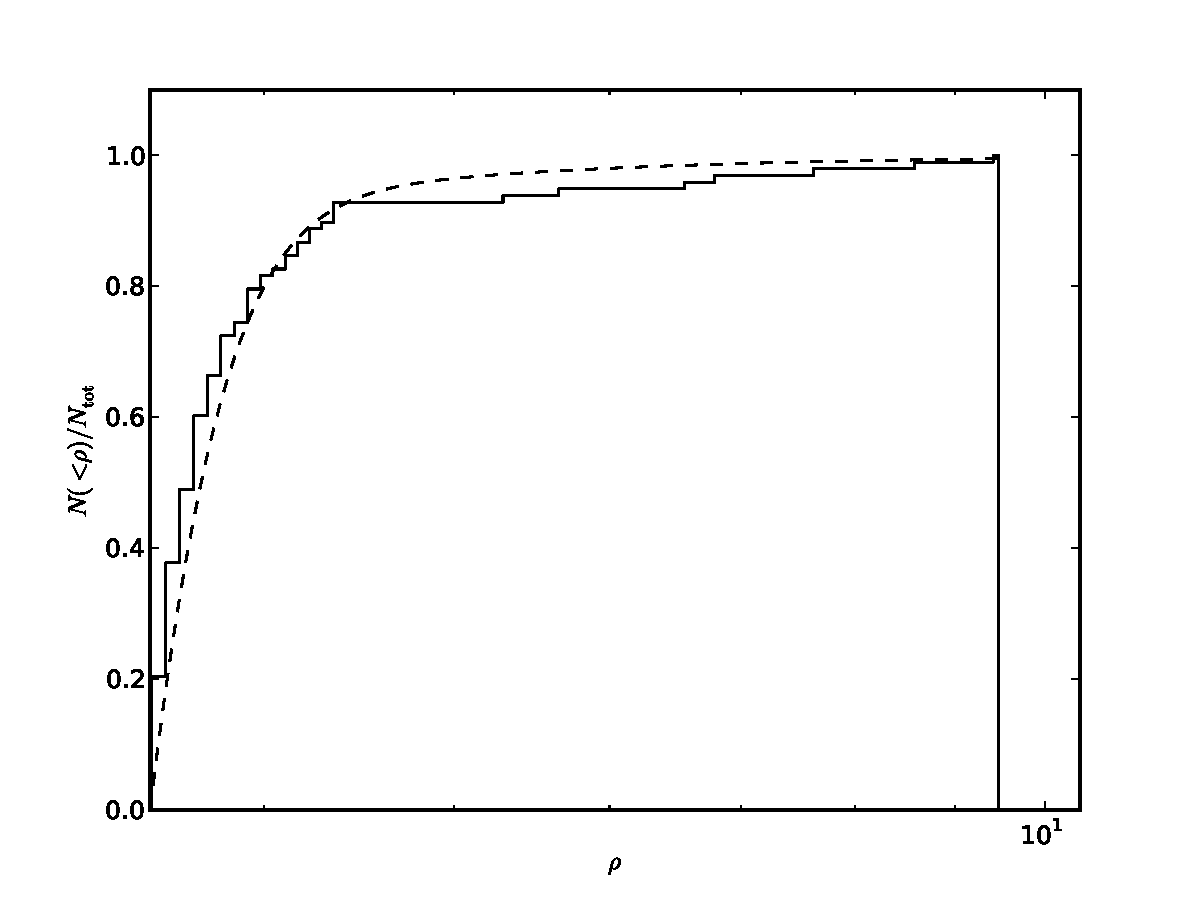
\includegraphics[width=\columnwidth]{data}
  \caption{\label{fig:analytic-data-cumulative} The cumulative
    distribution of the ranking statistics for the synthetic data used
    to test the formalism on the model from \S
    \ref{sec:analytic-GW-example}.  The solid line gives the
    cumulative distribution of the synthetic data; the dashed line
    gives the theoretical cumulative distribution for the models in
    Eqs.~\eqref{eq:analytic-background-rate} and
    \eqref{eq:analytic-foreground-rate} combined with $R_f = 10.4$ and
    $R_b = 95.1$.}
\end{figure}

In Figure \ref{fig:analytic-rate-recovery}, we show the marginalized
posterior densities for the foreground and background rates.  (Refer
to Eq.~\eqref{eq:rate-shape-posterior}.)  Figure
\ref{fig:analytic-rate-foreground-probs} shows the posterior
foreground probability for each event marginalized over all other
events' types and the foreground and background rates.

\ilya{Now, one interesting question that Fig.~3 brings to mind is the
  following: if we only used "gold-plated" events (say, those with
  $p(x|fore)/p(x|back)>0.99$, how much worse / more uncertain would
  the rate estimation be?]}

\begin{figure}
  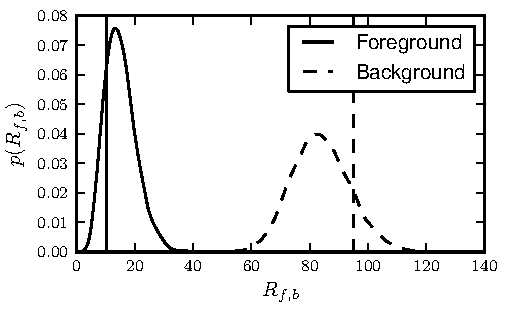
\includegraphics[width=\columnwidth]{rates}
  \caption{\label{fig:analytic-rate-recovery} The marginalized
    posterior densities for $R_f$ (solid line) and $R_b$ (dashed line)
    for the analytic model discussed in \S
    \ref{sec:analytic-GW-example}.  The vertical lines indicate the
    ``true'' values used to generate the synthetic data set.  Both the
    true foreground and background rates lie well within the
    probability envelope for $R_f$ and $R_b$.}
\end{figure}

\begin{figure}
  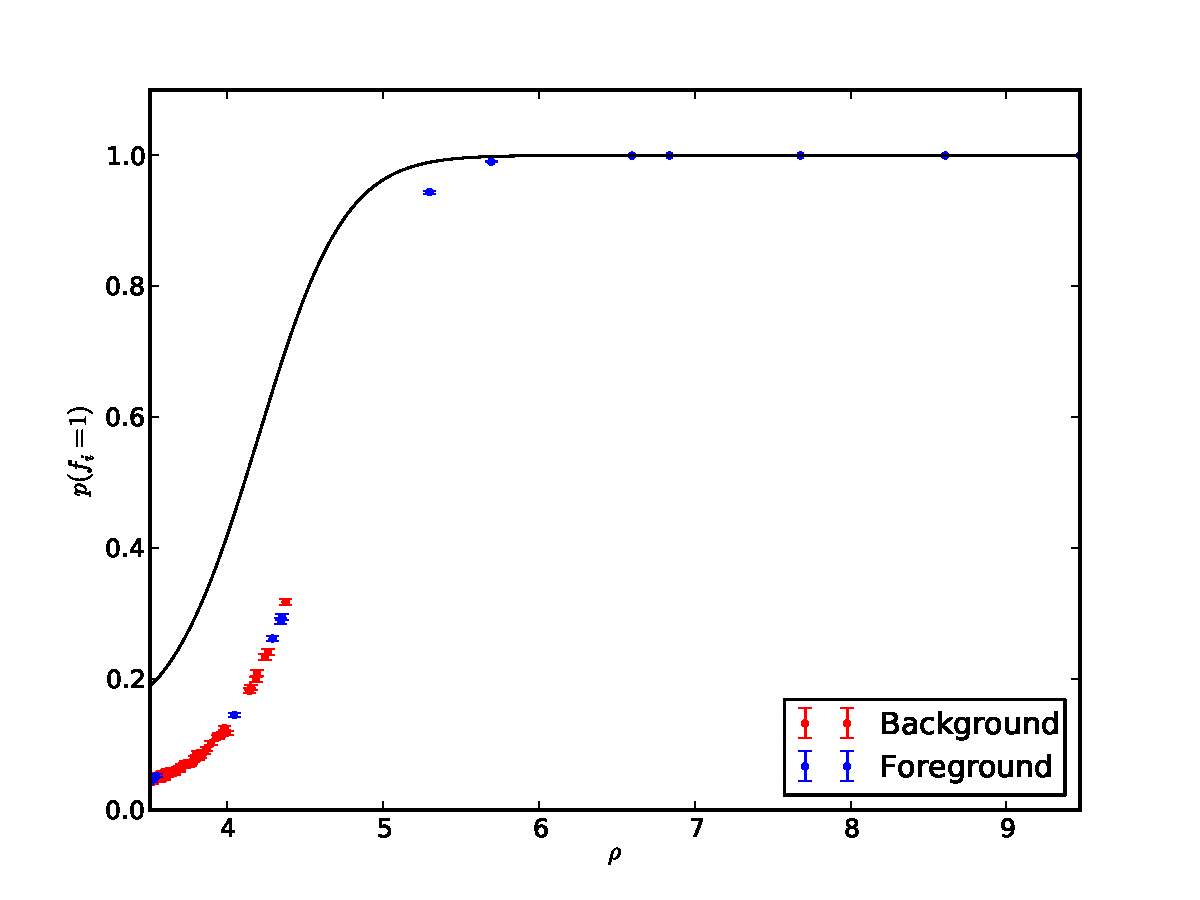
\includegraphics[width=\columnwidth]{pfore}
  \caption{\label{fig:analytic-rate-foreground-probs} Foreground
    probability for each event in the synthetic data set of \S
    \ref{sec:analytic-GW-example} marginalized over all other
    parameters (errorbars are one standard deviation).  True
    foreground events are in dark grey, background events in light
    grey.  Even though our method cannot identify the status of most
    events with confidence, it can still correctly estimate the rates
    (Figure \ref{fig:analytic-rate-recovery}).}
\end{figure}

\subsection{Gravitational Waves With Overlapping Templates}
\label{sec:gw-overlapping-template}

In \S~\ref{sec:analytic-GW-example} we assumed that the overlap
between different templates in the template bank was negligible, so
the SNRs recovered by different templates are independent random
variables.  In fact, template banks are not constructed in this way
\citep[e.g.,][]{Owen:1998dk,Ajith:2008}, because signals could fall in
the gaps between the non-overlapping templates.  We can model this
effect by assuming that a template bank of $N$ actual templates will
behave as if it had $N_\mathrm{eff}$ \emph{independent} templates.
Rather than pre-computing $N_\mathrm{eff}$, we can fit for it as a
shape parameter.  That is, we assume that $\theta =
\{N_\mathrm{eff}\}$ is a shape parameter for the background cumulative
distribution:
\begin{equation}
  \hat{B}\left(x, N_\mathrm{eff}\right) = \frac{\left( 1 + \erf\left(
    \frac{x}{\sqrt{2}} \right) \right)^{N_\mathrm{eff}} - \left( 1 +
    \erf\left( \frac{\xmin}{\sqrt{2}} \right)
    \right)^{N_\mathrm{eff}}}{2^{N_\mathrm{eff}} - \left( 1 +
    \erf\left( \frac{\xmin}{\sqrt{2}} \right) \right)^{N_\mathrm{eff}} }.
\end{equation}

Results from such an analysis on the data in
\S~\ref{sec:analytic-GW-example} appear in Figures \ref{fig:rates-nt}
and \ref{fig:ntemplates}.  Recall that the parameters used to generate
this data set are $R_f = 10.4$, $R_b = 95.1$, and $N_\mathrm{eff} =
1000$.  We use a flat prior on $N_\mathrm{eff}$.  Both the rates and
the number of effective templates are recovered without significant
loss of accuracy relative to the fixed $N_\mathrm{eff}$ situation in
\S~\ref{sec:analytic-GW-example}.

\ilya{[Again, I think we need to explicitly compare this method with
    two alternatives.  Alternative one is the loudest event statistic.
    Alternative two is just counting gold-plated events, and dividing
    the volume in which we are sensitive to them by their number.  In
    principle, alternative one should be suboptimal when the number of
    events is more than 0 or 1, while alternative two should be OK
    when the number of events is large, but error-prone otherwise.
    But if we want people to use this technique, we have to defend the
    point that there is a regime where it is clearly superior (and say
    what that regime is).]}

\begin{figure}
  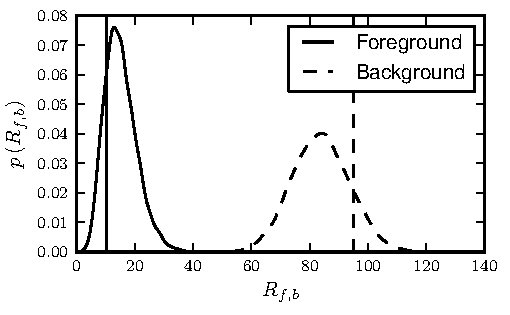
\includegraphics[width=\columnwidth]{rates-nt}
  \caption{\label{fig:rates-nt} The foreground (solid lines) and
    background (dashed lines) rate posterior, marginalized over all
    flags and the $N_\mathrm{eff}$ parameter, for the gravitational
    wave template detection scenario with overlapping templates
    discussed in \S \ref{sec:gw-overlapping-template}.  The true
    values of the rates, $R_f = 10.4$ and $R_b=95.1$, are indicated
    with vertical lines.  The distributions are not significantly
    wider than those of Figure \ref{fig:analytic-rate-recovery}, in
    spite of the extra parameter.}
\end{figure}

\begin{figure}
  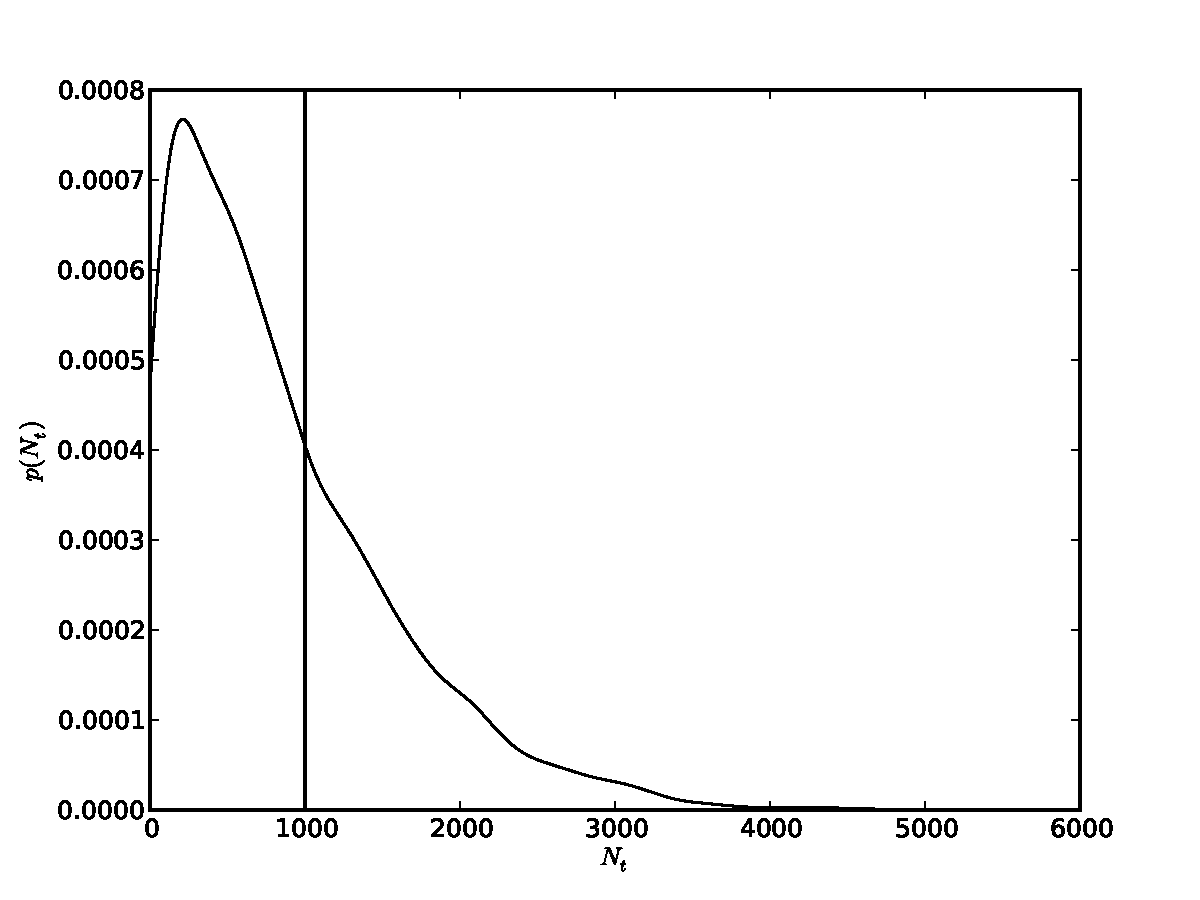
\includegraphics[width=\columnwidth]{ntemplates}
  \caption{\label{fig:ntemplates} The posterior on the number of
    effective templates, $N_\mathrm{eff}$, for the model and data
    discussed in \S \ref{sec:gw-overlapping-template}, marginalized
    over all state flags and rates.  The true value, $N_\mathrm{eff} =
    1000$, is indicated by the vertical line.}
\end{figure}

\subsection{Star Cluster Parameters With Background Contamination}
\label{sec:star-cluster}

\will{Look up von Hippel paper about Bayes 9, the cluster isochrone
  fitting software---we should cite, since our approach to cluster
  membership.}

Our final example concerns fitting for the location and shape
parameters of a cluster of stars observed on top of a stellar
background with a density gradient.  In this example, stars are either
members of the cluster (i.e.~foreground) or background contamination,
with a spatially varying density (i.e.~our rate functions are
two-dimensional).  We assume that a star cluster has a Plummer
surface-density profile \citep{Plummer1911,Aarseth1974},
\begin{equation}
  \label{eq:plummer-surface-density}
  \hat{f}(\vec{x}, \theta) = \frac{1}{\pi r_0^2 \left( 1 +
    \frac{\left| \vec{x} - \vec{x}_0 \right|^2}{r_0^2} \right)^2},
\end{equation}
where $\vec{x}_0$ is the location on the sky of the center of the
cluster, $r_0$ is a radial scale parameter, and $\vec{x} = \left( x, y
\right)$ is the position on the sky.  We assume a square observational
domain\footnote{The observational domain is not infinite, so the
  normalization of the cluster density in
  Eq.~\eqref{eq:plummer-surface-density} is not quite correct.  In our
  modeling we properly take this into account, but for simplicity here
  we ignore it.}, $\vec{x} \in [0,1]^2$, and a background that has a
density gradient at an arbitrary orientation with respect to the
observational axes:
\begin{equation}
  \hat{b}\left(\vec{x}, \theta\right) = 1 + \vec{\gamma} \cdot \left(
  \vec{x} - \vec{x}_{1/2} \right),
\end{equation}
where $\vec{\gamma}$ is the gradient, and $\vec{x}_{1/2} = [1/2, 1/2]$
is the centroid of the observational domain.  \ilya{[I think that if
    the domain is finite, the previous equation is only normalized for
    all $\vec{\gamma}$ if $\vec{x}_{1/2}$ is in the center of a
    symmetric domain (as it happens to be in this case).]}  \will{Yes,
  as you say, this function is only normalized for $\vec{x}_{1/2}$ is
  the center, and also for small enough $\vec{\gamma}$; both of these
  conditions obtain here.}  

We use simulated data drawn from our model with parameters
\begin{equation}
\label{eq:true-cluster-parameters}
\theta_0 \equiv \left\{ x_0, y_0, r_0, \gamma_x, \gamma_y \right\} =
\left\{ \frac{1}{2}, \frac{1}{2}, 0.18, -\frac{1}{2},
\frac{1}{2} \right\},
\end{equation}
with $R_f = 1000$ and $R_b = 10000$.  For this set of parameters, the
average density of the background and the peak density of the cluster
are comparable; there are an order of magnitude more background stars
than cluster stars in the field.  Figure \ref{fig:sky-density} shows
the density of stars (cluster and background) on the sky for our
particular data set.

\begin{figure}
  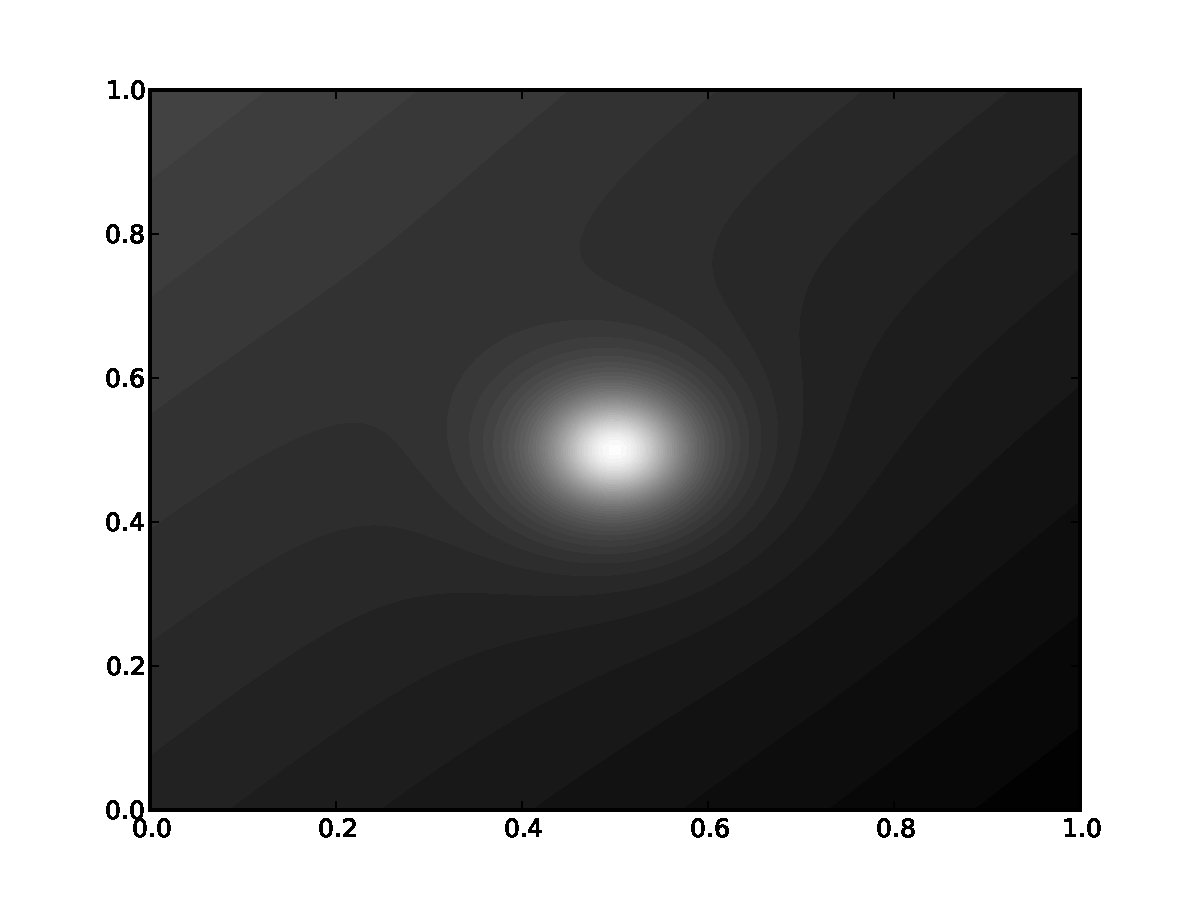
\includegraphics[width=\columnwidth]{sky-density}
  \caption{\label{fig:sky-density} The density contours on the sky of
    our synthetic data set of cluster and background stars for the
    parametrs in Eq.~\eqref{eq:true-cluster-parameters}.  There are a
    factor of 10 more stars (10000) in the background than in the
    cluster (1000), but the average density of cluster and background
    stars is similar.}
\end{figure}

To analyze our synthetic data set, we analytically marginalized over
the state flags (i.e.~cluster membership), using the likelihood in
Eq.~\eqref{eq:rate-shape-posterior}.  We did this to take advantage of
the \textit{emcee} sampler of \citet{ForemanMackey2012}, which
requires all parameters to be in $\mathbb{R}$.  We applied a prior on
the shape parameters that is flat in $\vec{x}_0$ and $\vec{\gamma}$,
and an (approximately) Jeffreys prior on $r_0$,
\begin{equation}
  p\left( r_0 \right) = \frac{\sqrt{R_f}}{r_0}.
\end{equation}
\ilya{[Why is this the Jeffreys prior (BTW, it's Jeffreys, or perhaps
    Jeffreys', but definitely not Jeffrey's ;) )?  It's not obvious
    why the prior on $r_0$ should depend on $R_f$?]}  \will{Here is
  the calculation:
\begin{equation}
  p\left( r_0 \right) = \sqrt{\left\langle \left(\frac{\partial \log
      \mathcal{L}}{\partial r_0 } \right)^2 \right\rangle} = \sqrt{
    R_f \left\langle \left(\frac{\partial \log\hat{f}}{\partial r_0
    }\right)^2 \right\rangle } = \sqrt{R_f \left\langle \left(
    \frac{2}{r_0} - \frac{4 r_0}{r^2 + r_0^2} \right)^2 \right\rangle}
  = \sqrt{\frac{ 4 R_f}{3 r_0^2}} \propto \frac{\sqrt{R_f}}{r_0}.
\end{equation}
Note that the calculation of the prior uses the likelihood before
analytical marginalization over the flags, $f_i$.  We are ignoring the
fact that $R_f$ and $r_0$ are correlated.  In truth, the Jeffreys
prior would be the determinant of the matrix built out of terms like
$\partial \log\mathcal{L} / \partial \theta_i \times \partial
\log\mathcal{L} /\partial \theta_j$, but let's not get carried
away\ldots.  As another aside, note that we could have predicted the
$1/r_0$ dependence because $r_0$ has units, so the only unit-invariant
prior is to be flat in $\log r_0$; I'm don't have a similar argument
for the appearance of the $\sqrt{R_f}$ factor.}  (Note that this
factor of $\sqrt{R_f}$ cancels with the Jeffreys prior on the rate,
$1/\sqrt{R_f}$; we have verified that the priors on these parameters
are irrelevant to our results, as would be expected from the
measurement of $\sim 1000$ foreground stars.)

Figure \ref{fig:sky-loc} shows the posterior for the location
parameters, $\vec{x}_0$; the center of the cluster is localized to
within about 10\% of the cluster scale.  Figure
\ref{fig:cluster-number} shows the posteriors inferred on the cluster
and background numbers, $R_f$ and $R_b$, and Figure
\ref{fig:cluster-scale} shows the posterior for the cluster's scale
parameter.  In spite of the significant background, the cluster scale
and total number are accurately recovered by our analysis.

\begin{figure}
  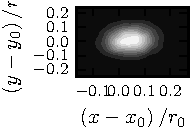
\includegraphics[width=\columnwidth]{sky_location}
  \caption{\label{fig:sky-loc} Contours of the posterior probability
    distribution for the center of the cluster, $\vec{x}_0$, in the
    example from \S~\ref{sec:star-cluster}.  The center $(x,y) =
    \left(x_0, y_0\right)$ is determined to within a few percent of
    the structural radius of the cluster, $r_0$ (see
    Eq.~\eqref{eq:true-cluster-parameters}). \ilya{[Given the cluster
        size of 0.1, it seems a bit surprising that the center is off
        by $\sim 0.05$...]}}
\end{figure}

\begin{figure}
  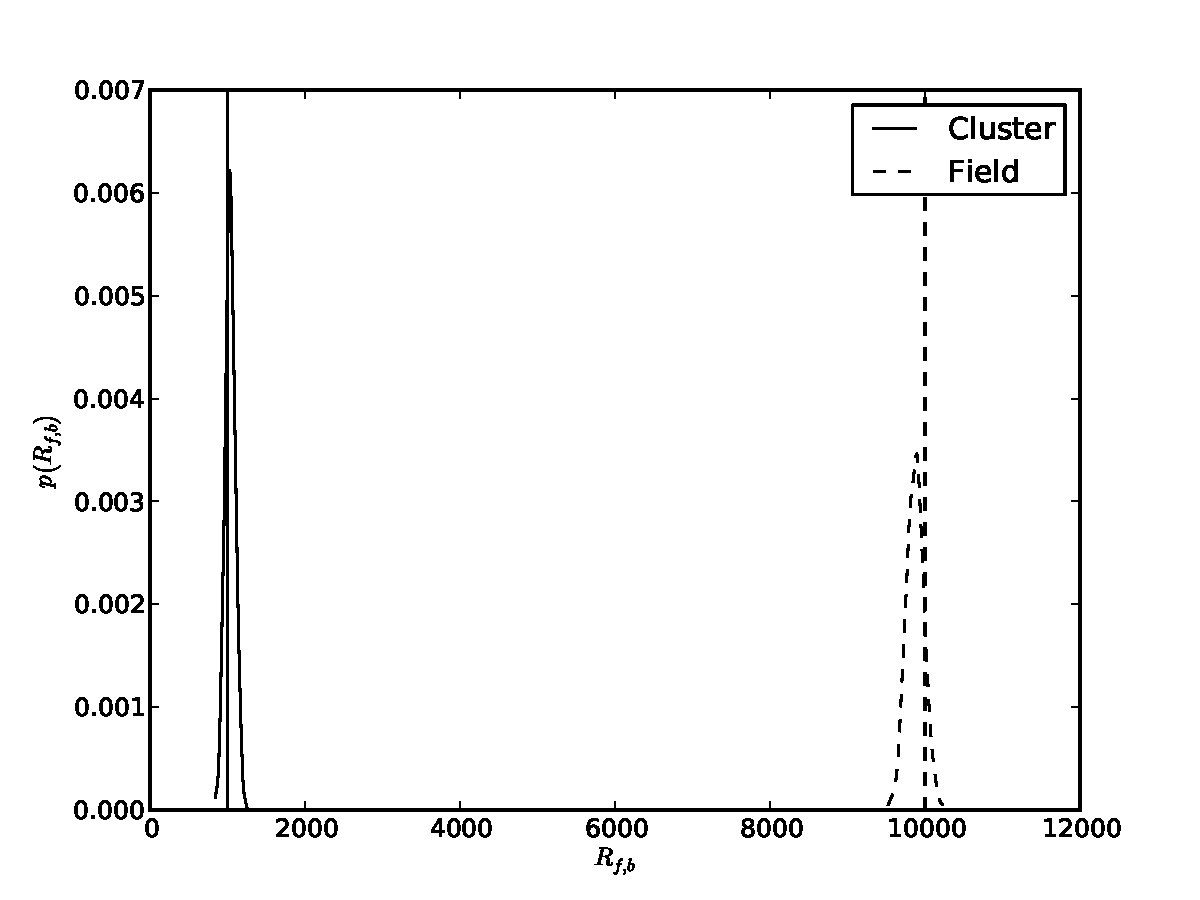
\includegraphics[width=\columnwidth]{numbers}
  \caption{\label{fig:cluster-number} Posterior densities for the
    number of stars in the cluster ($R_f$) and in the field ($R_b$) in
    the example from \S~\ref{sec:star-cluster}.  Vertical lines
    indicate the true values (see
    Eq.~\eqref{eq:true-cluster-parameters}). }
\end{figure}

\begin{figure}
  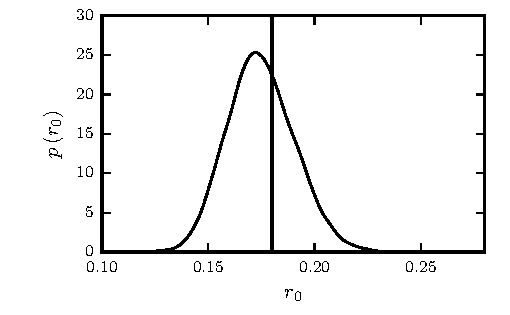
\includegraphics[width=\columnwidth]{scale}
  \caption{\label{fig:cluster-scale} Posterior density for the scale
    parameter for the cluster, $r_0$, from the example in
    \S~\ref{sec:star-cluster}.  The true value is indicated by the
    vertical line (see Eq.~\ref{eq:true-cluster-parameters}).
    \ilya{[Perhaps combine Figs.~8 and 9 (put an extra scale for $r_0$
        at the top of 8?]} }
\end{figure}

\section{Conclusion}

Separating classes of events

Comments on background probability estimation -- Cannon et al. in
prep.

Relevance (vs. loudest statistic, or frequentist approach using only
gold-plated events)

\begin{acknowledgments}
  We thank Kipp Cannon, Chad Hanna, Drew Keppel, and Richard
  O'Shaughnessy for discussions and suggestions about this manuscript.
\end{acknowledgments}

%%%%%%%%%%%%%%%%%%%% Bibliography 
\bibliographystyle{apsrev4-1} \bibliography{many}

\end{document}
